\titleformat
{\chapter} % command
[display] % shape
{\bfseries\Huge} % format
{ } % label
{2ex} % sep
{
    %\vspace{1ex}
} % before-code
[ \vspace{0ex}
] % after-code


\chapter[scPRINT: pre-training on 50 million cells allows robust gene network predictions]{scPRINT: pre-training on 50 million cells allows robust gene network predictions}
\label{article1}

\section{Summary}

A cell is governed by the interaction of myriads of macromolecules. Inferring such a network of interactions has remained an elusive milestone in cellular biology. Building on recent advances in large foundation models and their ability to learn without supervision, we present \gls{scPRINT}, a large cell model for the inference of gene networks pre-trained on more than 50 million cells from the \gls{CxG} database. Using innovative pretraining tasks and model architecture, \gls{scPRINT} pushes large transformer models towards more interpretability and usability when uncovering the complex biology of the cell. Based on our atlas-level benchmarks, \gls{scPRINT} demonstrates superior performance in gene network inference to the \gls{SOTA}, as well as competitive zero-shot abilities in denoising, batch effect correction, and cell label prediction. On an atlas of \gls{BPH}, \gls{scPRINT} highlights the profound connections between ion exchange, senescence, and chronic inflammation.

\section{Introduction}

Understanding the cellular mechanism is considered a milestone in biology, allowing us to predict cell behavior and the impact of drugs and gene knock-outs\citep{lahnemannElevenGrandChallenges2020, roohaniPredictingTranscriptionalOutcomes2024,gonzalezCombinatorialPredictionTherapeutic2024,haradaDistinctCoreRegulatory2022a,haradaLeukemiaCoreTranscriptional2023}. A cell is regulated by a complex interplay of myriads of macromolecules that define its state. We can simplify these interactions via a \gls{GN}\citep{badia-i-mompelGeneRegulatoryNetwork2023} (GN). Many approaches have been developed to infer these networks, focusing on \gls{TF}-to-gene links using single-cell omics data modalities like \gls{scRNA-seq} and \gls{scATAC-seq}\citep{littmanSCINGInferenceRobust2023,aibarSCENICSinglecellRegulatory2017,bravogonzalez-blasSCENICSinglecellMultiomic2023,suInferringGeneRegulatory2024,ganInferringGeneRegulatory2024, raharinirinaInferringGeneRegulatory2021,chenGraphAttentionNetwork2022,wangDictysDynamicGene2023,zhangInferenceCellTypespecific2023,wangInductiveInferenceGene2020,kamimotoDissectingCellIdentity2023,shuModelingGeneRegulatory2021}. This gene network subset regulating the cell gene expression levels is often called a \gls{GRN}. However, many other gene products than \gls{TF}s impact \gls{RNA} abundances in the cell, like \gls{RNA}-\gls{RNA} and protein-\gls{TF} interactions\citep{boijaTranscriptionFactorsActivate2018,gretafriarItTakesThree2023,oksuzTranscriptionFactorsInteract2023,talukdarTranscriptionalCoactivatorsEmerging2023,statelloGeneRegulationLong2021}. Most \gls{GRN} inference methods do not scale to the number of genes and cells present in single-cell \gls{RNA} datasets, and they need many cells, thus impairing their ability to reconstruct cell-state-specific networks. Other methods consider datasets where differentiating cells can be ordered temporally to predict more causal \gls{GRN}s. While this approach is interesting, temporal ordering is often hard to predict\citep{wangDictysDynamicGene2023,wangDecipheringDriverRegulators2023}.

Benchmarks like BeeLine\citep{pratapaBenchmarkingAlgorithmsGene2020} and MCalla et al.\citep{mccallaIdentifyingStrengthsWeaknesses2023} have shown that despite the existence of many methods, \gls{GN} inference remains a challenging problem. Indeed, it is underconstrained and has limited prior knowledge. New foundational models trained on tens of millions of measurements could help solve these difficulties. Transformers like \gls{BERT}\citep{vaswaniAttentionAllYou2023,devlinBERTPretrainingDeep2019} have gained traction in computational biology and have held promise to learn a model of the cell that would translate across many tasks of cellular biology, such as cell type annotation, batch-effect correction, perturbation prediction, and gene network inference\citep{theodorisTransferLearningEnables2023}. Among them, \gls{scGPT}\citep{cuiScGPTBuildingFoundation2024} got much attention, proposing a novel encoding of genes and their expression, a new pretraining methodology similar to autoregressive pretraining in language models, and the possibility of extracting \gls{GRN} from its model (see ~\ref{sec:methodsprint}. methods).

Inspired by these efforts, we propose \gls{scPRINT} (single-cell PRe-trained Inference of Networks with Transformers), a foundation model designed for gene network inference. \gls{scPRINT} brings inductive biases and pretraining strategies better suited to \gls{GN} inference while answering issues in current models (see ~\ref{sec:suppscprint}. Supplementary Table S1). \gls{scPRINT} outputs cell type-specific genome-wide gene networks but also generates predictions on many related tasks, such as cell annotations, batch effect correction, and denoising, without fine-tuning.

We extensively benchmark \gls{scPRINT} on challenging gene network inference tasks, from literature-based networks to cell type-specific ones generated via orthogonal sequencing methods. We show that \gls{scPRINT} outperforms the \gls{SOTA} on most of these atlas-level benchmarks. In addition, our model focused on \gls{GN} inference, is also competitive on a compendium of tasks like denoising, cell type prediction, and embedding with batch effect correction. This suggests that by learning a cell model, \gls{scPRINT} gains zero-shot abilities in many tasks of cellular biology. 
We use \gls{scPRINT} to analyze an atlas of normal and senescent prostate tissues where we identify rare cell populations with early markers of the \gls{TME} in B-cells. In fibroblasts, we study gene networks and recover known hubs such as PAGE4, linking the senescence of fibroblasts to changes in the \gls{ECM} and downstream inflammation. We find key interconnected pathways of the oxidative stress response and extracellular matrix building via metal and ion exchange in the gene network of \gls{BPH}-associated fibroblasts. We also show that healthy and disease-related cells exhibit different network patterns, demonstrating that \gls{scPRINT} can help identify novel pathways and targets while considering them in their specific cellular and molecular contexts.

\gls{scPRINT}\citep{kalfonCantinilabScPRINT2025} (\url{https://github.com/cantinilab/scPRINT}) is a fast and open-source tool that can be readily integrated into the bioinformatics pipeline. We make public the code and model weights, but also the pretraining strategies, datasets, and our own dataloader for use with vast training sets like the \gls{CxG} databas\citep{programCZCELLxGENEDiscover2023}. We also release a Gene Network benchmarking suite: \emph{BenGRN}\citep{kalfonJkobjectBenGRNAwesome2025} and \emph{GrnnData}\citep{kalfonCantinilabGRnnData2025}. 

\section{Results}

\subsection{scPRINT: a scRNAseq foundation model for gene network inference}

We propose \gls{scPRINT} (Figure ~\ref{fig:firstscprint}A), a \gls{SOTA} bidirectional transformer designed for cell-specific gene network inference at the scale of the genome. \gls{scPRINT} is trained with a custom weighted-random-sampling method\citep{jeremiekalfonTrainingFoundationModels} over 50 million cells from the \gls{CxG}\citep{programCZCELLxGENEDiscover2023} database from multiple species, diseases, and ethnicities, representing around 80 billion tokens (see ~\ref{sec:methodsprint}. Methods). We train \gls{scPRINT} at various scales (from 2M to 100M parameters) and very efficiently by using flashattention2\citep{daoFlashAttention2FasterAttention2023}, e.g., only requiring an A40 \gls{GPU} for 48 hours to train our medium model, significantly reducing the barrier to entry for any computational biology lab (see ~\ref{sec:suppscprint}. Supplementary Table S2).

To push \gls{scPRINT} to learn meaningful \gls{GN}s and their underlying cell model, we design a unique set of pretraining tasks, as well as expression encoding and decoding schemes (Figure ~\ref{fig:firstscprint}B).

\gls{scPRINT}'s pretraining is composed of three tasks which loss are added and optimized together: a denoising task, a bottleneck learning task, and a label prediction task. The objective is to let \gls{scPRINT} learn to represent meaningful gene connections while also endowing it with a breadth of zero-shot prediction abilities.

Indeed, similarly to ADImpute\citep{leoteRegulatoryNetworkbasedImputation2022,eraslanSinglecellRNAseqDenoising2019}, we expect a good gene network to help denoise an expression profile by leveraging a sparse and reliable set of known gene-gene interactions.

We implement this denoising task as the upsampling of transcript counts per cell (see ~\ref{sec:methodsprint}. Methods). While most other methods have been using masking as a pretraining task, our method is related to the downsampling and masking task of scFoundation\citep{haoLargescaleFoundationModel2024}. We show that this strategy performs better than masked language modeling and gives \gls{scPRINT} the ability to upsample any expression profile.

In addition, we expect that a cell model tasked to compress expression profiles into embeddings can learn the regularities of modules and communities of gene networks. Therefore, the bottleneck learning task drives \gls{scPRINT} to generate an embedding and a cell expression profile from its embedding only. The embedding is generated by \gls{scPRINT} and is used again, this time without the cell expression values, to regenerate the true profile (see ~\ref{sec:methodsprint}. Methods).

Finally, the cell's gene network should represent the cell state and its different phenotypic facets. Effectively, \gls{scPRINT} generates not just one embedding per cell but multiple. A hierarchical classifier is then applied to each distinct cell embedding to predict its associated class, such as cell type, disease, sex, organism, ethnicity, and sequencing platform. The embeddings thus become disentangled, each representing a specific facet of the cell state\citep{piranDisentanglementSinglecellData2024}. This last training task pushes the large cell model and its gene network to represent the cell state.

\begin{figure}[H]
    \centering
    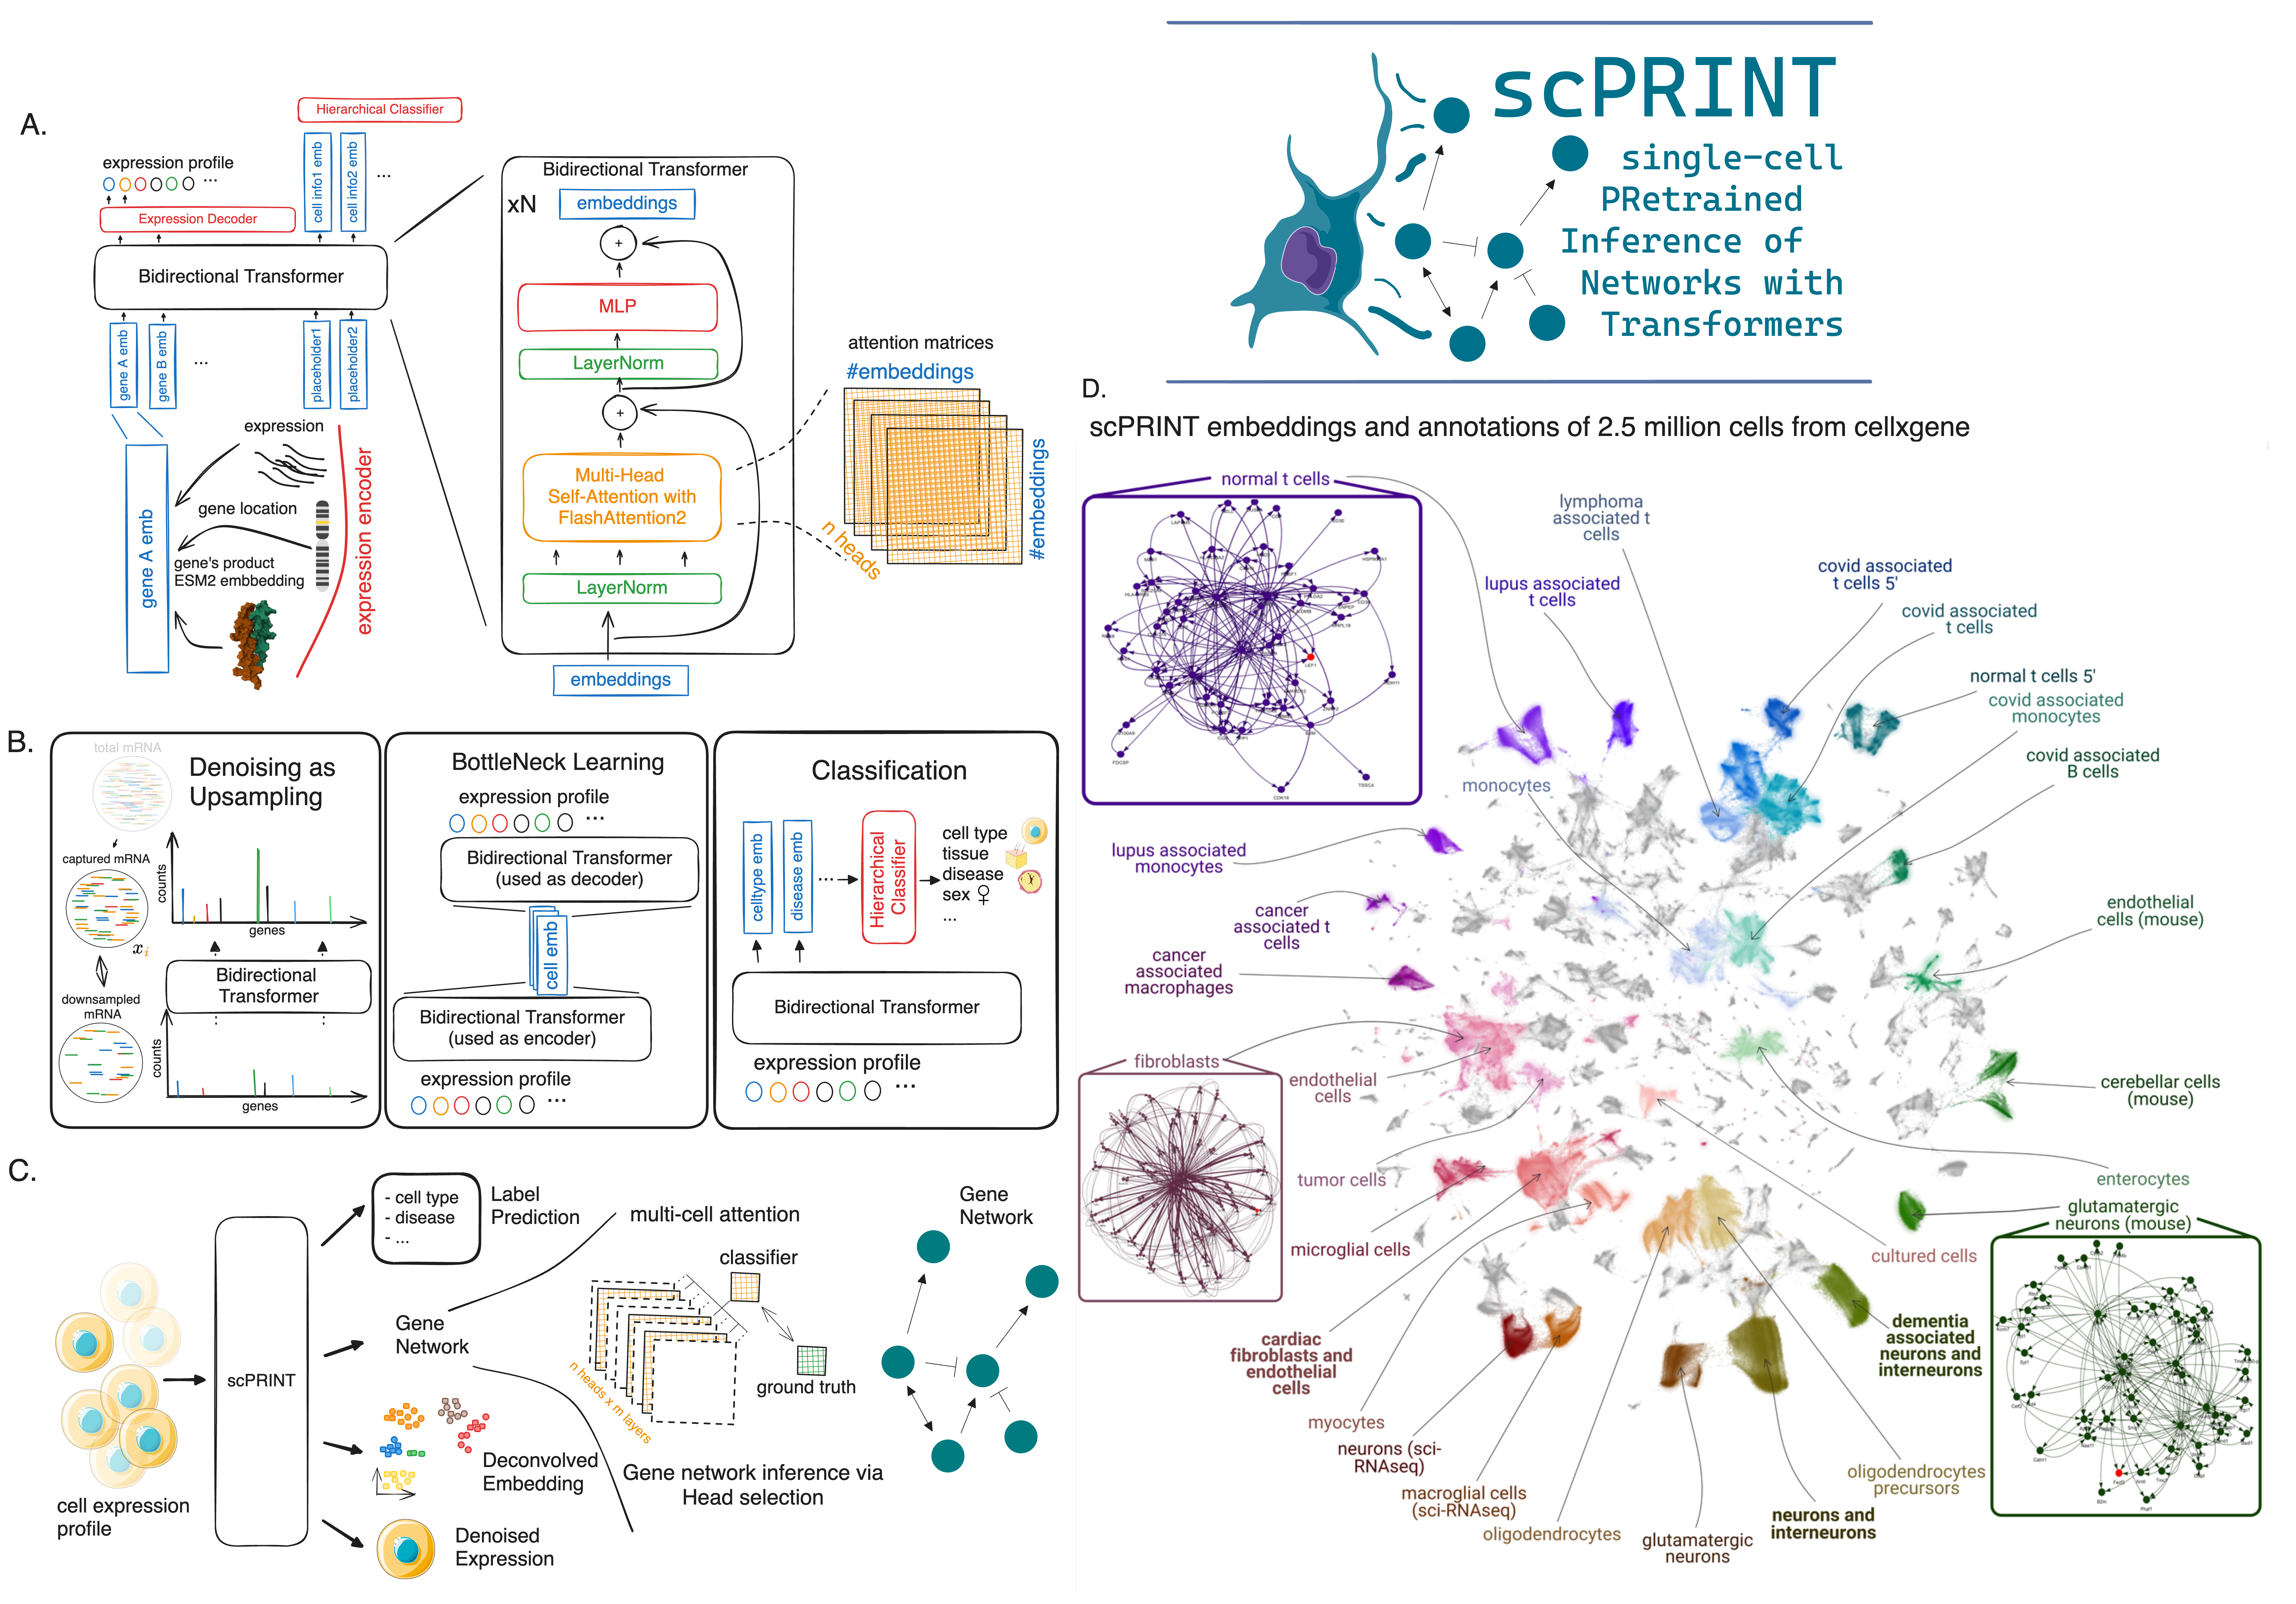
\includegraphics[width=0.9\textwidth]{figures/scprint/figure1}
    \caption[presentation of the scPRINT model and training]{(a) Schematic representation of \gls{scPRINT} with its bidirectional encoder, gene expression embedding encoding via gene location, matched protein \gls{ESM}2 embedding, and gene expression. (b) \gls{scPRINT} pre-training tasks: Denoising task whose goal is to recover the known transcriptomic profile from a purposefully downsampled expression profile. Bottleneck learning reconstructs the expression of requested genes using only their cell embedding. The same model is used for both The encoding and decoding steps. Hierarchical classification is achieved by applying a hierarchical classifier to each disentangled embedding. This pushes the first embedding to contain cell type info, the second embedding to contain disease info, and so on (see ~\ref{sec:methodsprint}. methods). (c) The different outputs in \gls{scPRINT}. \gls{scPRINT} generates label predictions of cell type, tissue, disease, sex, sequencer, ethnicity, and organism. \gls{scPRINT} generates multiple embeddings (which we call disentangled embedding), a general one, as well as a specific embedding for each class. \gls{scPRINT} also generates a reconstructed expression profile at any requested sequencing depth (i.e., total transcript count) (denoising). \gls{scPRINT} also generates a Gene Network by selecting and combining various attention heads into a gene x gene matrix. (d) Example of a \gls{scPRINT} output from a random subset of 2.5 million cells from the \gls{CxG} database. Embeddings and labels are generated by \gls{scPRINT}, together with the example cell type-specific gene networks. We show only subparts of the networks extracted from a central node, represented in red.}
    \label{fig:firstscprint}
\end{figure}

Thanks to the \gls{CxG} database requirement for complete annotations and our innovative hierarchical classifier, we have added label prediction as part of the pretraining of \gls{scPRINT}. While the assumption is that in other modalities, the scarcity and noisiness of such labels make it infeasible, we show that this approach is a net positive in our case (see ~\ref{sec:suppscprint}. Supplementary Table S3, ~\ref{sec:methodsprint}. Methods). Indeed, it helps us disentangle the various cell embeddings and performs zero-shot predictions on unseen datasets. These disentangled embeddings are opening a future possibility to perform counterfactual generation: mixing embeddings representing different facets of cell states, e.g., fibroblast + cancer + pancreas tissue + female, to generate novel unseen expression profiles.

\gls{scPRINT} converts the gene expression of a cell to an embedding by summing three representations or tokens: its id, expression, and genomic location (Figure ~\ref{fig:firstscprint}A, see ~\ref{sec:methodsprint}. Methods). \gls{scPRINT} encodes the gene IDs using protein embeddings. This gene representation is made using the \gls{ESM}2\citep{rivesBiologicalStructureFunction2021} amino-acid embedding of its most common protein product (see ~\ref{sec:suppscprint}. Supplementary Figure S1). First proposed in \gls{UCE}\citep{rosenUniversalCellEmbeddings2023}, the model learns to leverage representations that can potentially apply to unseen genes and species, using the structural and evolutionary conservation of the sequence encoded by \gls{ESM}2. While drastically reducing the number of weights used in the model compared to \gls{scGPT} and Geneformer (see ~\ref{sec:methodsprint}. Methods), this representation also contains some priors needed to infer protein-protein\citep{huImprovingProteinproteinInteraction2024} interactions (Figure ~\ref{fig:firstscprint}A). 

The gene's expression is tokenized via a \gls{MLP} using log-normalized counts. This \gls{MLP} lets the model learn a metric behind gene expression, whereas \gls{scGPT} and Geneformer apply a specific prior for the encoding of their gene expression (see ~\ref{sec:methodsprint}. Methods).

Finally, we help the model know that genes with similar locations tend to be regulated by identical \gls{DNA} regions, using the positional encoding of their location in the genome (see ~\ref{sec:methodsprint}. Methods).

These three embeddings are summed and then concatenated across all the genes expressed in a cell together with additional placeholder cell embeddings to form the transformer model's input.

\gls{scPRINT} is pretrained using 2,200 randomly selected expressed genes in a cell profile. If a cell doesn't have enough expressed genes, the list is padded with randomly selected unexpressed genes. A context of 2200 genes, while not genome-wide, captures all the expressed genes in more than 80\% of the cell profiles in the \gls{CxG} database. We also show that \gls{scPRINT} can make predictions on much larger sequences of genes at inference time without using attention approximation methods\citep{choromanskiRethinkingAttentionPerformers2022}.

Using unexpressed genes, combined with the denoising task, let \gls{scPRINT} discriminate the true zeros from dropouts in \gls{scRNA-seq}47. The expression decoder of \gls{scPRINT} further helps model this statistic of the data. It is a zero-inflated negative binomial graphical model inspired by previous literature in single-cell \gls{RNA-seq} modeling48. Here, the loss (also used for bottleneck learning) is thus the log-likelihood of the gene expression given the distribution parameters.

As shown in Figure ~\ref{fig:firstscprint}C, at inference time, \gls{scPRINT} can generate multiple outputs across any \gls{scRNA-seq}-like cellular profile of various mammalian species without fine-tuning. Figure ~\ref{fig:firstscprint}D shows \gls{scPRINT}'s prediction at the scale of an atlas of 2M randomly sampled cells from \gls{CxG}. From its pre-training, \gls{scPRINT} performs denoising, label prediction, and cell embedding without fine-tuning. However, a critical emergent output of \gls{scPRINT} is its cell-specific gene networks. Following a similar approach to \gls{ESM}2, we generate cell-level gene networks via the bidirectional transformer's input-wise weighted matrices, called attention matrices -or heads-. They represent general gene-gene connections and can be subsetted to \gls{TF}-gene connections (i.e., \gls{GRN}s). Remarkably, we made this approach scalable enough to compute attention heads-based gene networks for 1 to 10,000 cells, at the genome scale, with commodity hardware and in a few minutes. These networks both showcase the ability of \gls{scPRINT} to model cellular biology and help make it a more explainable tool for the community, showing the network assumptions made during inference. The attention heads are either all aggregated by averaging or can be selected to better reflect connections of interest (Figure ~\ref{fig:firstscprint}C). This is done using the average of the heads most correlated with literature or perturbation-based ground truth networks. Finally, while we do not assess \gls{scPRINT}'s ability to model inhibition due to the scarcity of such annotations, we leave open the possibility of using our head selection technique for such a task. 

Similarly to what has already been done in \gls{ESM}2 and the Large Language Model literature\citep{abnarQuantifyingAttentionFlow2020,clarkWhatDoesBERT2019a,bibalAttentionExplanationIntroduction2022}, we deeply investigate the meaning of attention matrices in the context of cellular biology, an aspect under-studied in the literature of foundation models applied to genomics. 

In the following sections, we benchmark \gls{scPRINT} on gene network inference against \gls{scGPT}, Deep\gls{SEM}\citep{shuModelingGeneRegulatory2021}, GENIE3\citep{huynh-thuInferringRegulatoryNetworks2010}, and Geneformer v2\citep{chenQuantizedMultitaskLearning2024}, the updated version of Geneformer. \gls{scGPT} and Geneformer v2 are highly cited and published transformer models for single-cell \gls{scRNA-seq}, mentioning the inference of gene interactions\citep{cuiScGPTBuildingFoundation2024}. Deep\gls{SEM} is an autoencoder model jointly learning its weights and a gene network matrix. GENIE3 generates networks via regression by finding the set of genes that best predict another gene's expression. It is one of the top-performing and most used methods for \gls{GRN} inference (see ~\ref{sec:methodsprint}. Methods). However, it suffers from very long run times and high memory requirements (see ~\ref{sec:suppscprint}. Supplementary Table S4).

\subsection{scPRINT recovers biological features in its gene networks}

We benchmark \gls{scPRINT} against the \gls{SOTA} based on whether their recovered networks contain meaningful biological knowledge. We consider two main benchmarking methodologies, one using a simulated expression profile from a well-established biological network. Because simulated data does represent real cell expression data (see ~\ref{sec:methodsprint}. Methods), our second and main approach focuses on biological features of a network inferred from real cell expression profiles. Indeed, we assume that a meaningful gene network should have some of its hub nodes being \gls{TF}s. \gls{TF}s should be more connected to their known target, on average. We should recover known gene-gene connections and expect enrichment of cell type-specific marker genes in the network.

We compare each gene network inference method's ability to recover a known network from 1000 simulated single-cell \gls{scRNA-seq} expression profiles generated by the Sergio \gls{ODE} model\citep{dibaeiniaSERGIOSingleCellExpression2020} from the ground truth network Regnetwork\citep{liuRegNetworkIntegratedDatabase2015} (see ~\ref{sec:methodsprint}. Methods). Only \gls{scPRINT} was able to recover meaningful connections (see ~\ref{sec:suppscprint}. Supplementary Table S5). One explanation is that through its training, \gls{scPRINT} has learned the common gene connections that also exist in the RegNetwork ground truth.

\begin{figure}[H]
    \begin{center}
        \includegraphics[width=0.8\linewidth] {figures/scprint/figure2}
    \end{center}
    \caption[Analysis of the gene networks generated by \gls{scPRINT}]{(a) We extract cell type-specific gene networks for each cell type in the dataset (n=26 cell types across 3 datasets). We perform Gene Set Enrichment Analysis (\gls{GSEA})\citep{subramanianGeneSetEnrichment2005a} on the network's nodes (n=4000 genes). We compute the ability of the edges to recover the Omnipath ground truth's connections. (b) Violin plot of the ten different \gls{AUPRC} and \gls{EPR} values obtained when comparing the inferred cell type-specific networks with the Omnipath network for \gls{scPRINT}: average of all attention heads, \gls{scPRINT} (genome): same \gls{scPRINT} version but computing a genome-wide gene network, \gls{scPRINT} (omnipath's heads): same \gls{scPRINT} version but with attention heads selected using a subset of omnipath, \gls{scGPT}, Deep\gls{SEM}, Geneformer v2, and GENIE3, when considering only \gls{TF}-gene connection or all gene-gene connections. (c) Violin plot of the average number of \gls{TF} with enrichment for their \gls{ENCODE} target in each cell-type-specific network. (d) Number of \gls{GN}s with a significant enrichment of \gls{TF}s and of their cell type's marker genes.}
    \label{fig:secondscprint}
\end{figure}

On gene network inference from real expression data, we noticed that depending on cell type and datasets, the different tools could vary greatly in the similarity of their \gls{GN}s to the Omnipath\citep{tureiOmniPathGuidelinesGateway2016} ground truth. Because of this, we focused our benchmark on three randomly selected test datasets of kidney, retina, and colon tissues comprising 26 cell types\citep{marshallHighresolutionSlideseqV2Spatial2022,wangSinglecellMultiomeHuman2022b,kongLandscapeImmuneDysregulation2023} (see ~\ref{sec:methodsprint}. Methods, per dataset results in \ref{sec:suppscprint}. Supplementary Figure S2). Of note is that we could not determine if these datasets were used during the training of \gls{scGPT} or Geneformer. 

We build one network per cell type, using the same 1024 cells and their 5000 most differentially expressed genes for all benchmarked methods. We evaluate the quality of the networks based on their overlap with Omnipath. We also compute the network enrichment for cell type markers, \gls{TF}s, and \gls{ENCODE} \gls{TF} targets using the prerank\citep{subramanianGeneSetEnrichment2005a} algorithm (Figure ~\ref{fig:secondscprint}A).

Although the \gls{scGPT} code mentions \gls{GRN} inference only using perturb-seq data, we reapply the same method without the perturbation-baseline comparison. This is to make it comparable with other benchmarked methods and because most of our datasets are not perturbation-based. Similar to what is presented in its paper, we use the mean of the attention matrices across cells and the four attention heads of the last layer of the human pre-trained model. We retain this method across our benchmarks for \gls{scGPT} (see ~\ref{sec:methodsprint}. Methods). We apply a similar strategy for Geneformer (see ~\ref{sec:methodsprint}. Methods).

For \gls{scPRINT}, we generate three network versions: one simply called \gls{scPRINT}, based on the average of all heads in the model. \gls{scPRINT} (omnipath's heads), based on the average of heads selected with our abovementioned head selection method inspired by \gls{ESM}2, and \gls{scPRINT} (genome), which is like the \gls{scPRINT} network but uses our method to generate genome-wide networks (see ~\ref{sec:methodsprint}. Methods) instead of using the 5000 most differentially expressed genes. Indeed, in transformer models, the choice of attention heads is important. Although transformers can learn the causal structure of their input, it has been shown that some attention heads, especially in larger networks, can become unused, containing predominantly random connections\citep{nichaniHowTransformersLearn2024}. Some work has been done at pruning these heads\citep{shimLayerwisePruningTransformer2021} or forcing a head selection mechanism during inference and training\citep{fedusSwitchTransformersScaling2022}. For \gls{scPRINT} (omnipath's heads), we select heads based on a linear classifier's prediction of the best set of heads to predict a subset of Omnipath (see ~\ref{sec:methodsprint}. Methods). Similarly to the \gls{scPRINT} network, these heads are then averaged to generate the \gls{scPRINT} (omnipath's heads) gene network. To perform this selection, we split the omnipath dataset into train/test and select heads, using 50\% of the ground truth and only the first cell type of each dataset. We then use the same combination of heads across all other cell types. This shows that our selection process builds consistent networks across cell types and parts of the ground truth. This innovative approach contrasts with previous ones like \gls{scGPT}'s and GENIE3 by using part of an available ground truth to select heads.

First, we look at how much information from Omnipath is contained in the inferred networks. Omnipath contains around 90,000 curated gene-gene connections, mainly from the literature. These connections are cell type agnostic, and most are \gls{TF} - gene. On this benchmark, we evaluate the networks based on \gls{AUPRC} and \gls{EPR}, two metrics often used in \gls{GRN} benchmarks\citep{pratapaBenchmarkingAlgorithmsGene2020} (see ~\ref{sec:methodsprint}. Methods), where we define our task as a binary classification of connections on all gene-gene pairs. Due to the row-wise normalization of networks generated by all methods, and because Omnipath has many sources with only a few targets (see ~\ref{sec:suppscprint}. Supplementary Figure ~\ref{fig:secondscprint}), we here use the transpose of our inferred networks when making comparisons with Omnipath (see ~\ref{sec:methodsprint}. Methods).
In Figure ~\ref{fig:secondscprint}B, we can see that \gls{scPRINT} (omnipath's heads) outperforms all methods on average across all cell types. While \gls{scPRINT} (omnipath's heads) uses some ground truth information to select its head, we see that \gls{scPRINT} still outperforms \gls{scGPT} and Geneformer v2 on the \gls{EPR} metric, showing that its top predicted edges more closely match the ground truth. 

\gls{AUPRC} results are very low overall because we do not expect most Omnipath connections to be present in the cell type's gene network, as many connections in Omnipath might only be true in some cellular contexts. Moreover, we do not expect most connections in our generated network to exist in Omnipath as it only contains a small fraction of all real gene-gene connections. Although overall \gls{AUPRC} values are small, we can see that both \gls{scGPT} and \gls{scPRINT} outperform the other methods in the number of connections recovered. Indeed, on average, \gls{scGPT} and \gls{scPRINT} respectively recover 42\% and 67\% more connections than GENIE3.

However, GENIE3 is often used by biasing the method to only predict \gls{TF}-gene connections (see ~\ref{sec:methodsprint}. Methods). This type of network, usually called a \gls{GRN}, is most often used, given the importance of \gls{TF}s in regulating gene expression. To compare the other methods to this \gls{GRN} version of GENIE3, we also use a \gls{GRN} version of their networks by subsetting them to \gls{TF}-gene connections only. In this context, all the methods significantly improve their predictions without altering their relative performances (Figure ~\ref{fig:secondscprint}B). This is unsurprising, considering that Omnipath is strongly biased towards \gls{TF}-gene interactions. 

Interestingly, we have seen that smaller \gls{scPRINT} models containing fewer heads perform better when taking the average of their heads. In contrast, head selection is often more advantageous in larger models with more heads (see ~\ref{sec:suppscprint}. Supplementary Table S6). As presented at the beginning of the results section, it might be that as models become larger and less regularized, some heads tend to become unused and contain mostly noise. As a consequence, a head selection is advantageous in larger models. 

We also expect biologically meaningful gene networks to have their central nodes enriched for \gls{TF}s. In addition, because these networks are cell type-specific, we expect their central nodes to be enriched for some marker genes of their associated cell types (see ~\ref{sec:methodsprint}. Methods). In this regard, both \gls{scGPT} and \gls{scPRINT} achieve very similar and strong network enrichment for \gls{TF}s compared to GENIE3, Deep\gls{SEM}, and Geneformer v2, whose networks are not enriched for \gls{TF}s (Figure ~\ref{fig:secondscprint}C).

Moreover, amongst the 178 cell types we have marker gene sets for in pangaloDB\citep{franzenPanglaoDBWebServer2019}, all methods find some enrichment, especially GENIE3 and \gls{scGPT} (see ~\ref{sec:methodsprint}. Methods). We notice that selecting heads based on Omnipath significantly improves \gls{scPRINT}'s network enrichment for cell-type markers. Of note, our goal is not to annotate cell types from the gene network but mainly to showcase the network's cell type specificity. 

Finally, we also examine how much the connections of each \gls{TF} are enriched for that \gls{TF}'s target. Here, \gls{scPRINT} overperforms all other methods (Figure ~\ref{fig:secondscprint}D). In the \gls{scPRINT} networks, 20\% of the Transcription Factors for which we have data on \gls{ENCODE} have connections significantly enriched for their \gls{ENCODE}-validated gene targets\citep{liberzonMolecularSignaturesDatabase2015}. Interestingly, only our large cell model achieved a great performance, and \gls{scGPT} did not display any enrichment across the 26 cell types assessed. While we acknowledge that \gls{ENCODE} is used in the Omnipath database, we cannot expect  Omnipath to represent the \gls{ENCODE} targets. Indeed, it combines and processes 57 additional data sources to build its consensus network.

\gls{scPRINT} (genome) has been added despite its performance not being comparable to other methods. Indeed, comparing its overlap with Omnipath is unfair as it includes many more genes and connections, many of which will have almost no data on this ground truth. While \gls{scPRINT} (genome) showcases our ability to generate genome-wide networks, it also shows strong performances in \gls{TF} enrichment and \gls{ENCODE} \gls{TF}-target enrichments. This highlights that even at such a large scale, networks generated by \gls{scPRINT} are enriched in biological knowledge gained solely from its pre-training tasks.

Overall, we have shown that \gls{scPRINT} generates, in one forward pass, cell type-specific gene networks that are biologically meaningful. We will now examine them using cell type-specific ground truths extracted from orthogonal experiments.

\subsection{scPRINT outperforms the state of the art on cell type-specific ground truths}

Although we have shown that our networks represent meaningful biology, the Omnipath ground truth is literature-based and not cell type-specific. Here, we use two different modalities, perturb-seq\citep{dixitPerturbseqDissectingMolecular2016}, and \gls{ChIP-seq}\citep{parkChIPSeqAdvantages2009}, as ground truths to compare predicted gene networks against.

In the MCalla et al.\citep{mccallaIdentifyingStrengthsWeaknesses2023} ground truth, \gls{ChIP-seq}uencing and perturb-seq are intersected to get at the small subset of possibly direct connections between \gls{TF}s and genes for both human and mouse embryonic stem cells (ESC) (Figure ~\ref{fig:third}A, see ~\ref{sec:methodsprint}. Methods). We have seen that these ground truth networks show a different pattern than literature-based networks (see ~\ref{sec:suppscprint}. Supplementary Figure S3). Some \gls{TF}s regulate only a few genes, whereas others are highly connected.

To generate our networks, we use as input one human and two mouse ESC \gls{scRNA-seq} datasets from MCalla et al. with the addition of another human dataset from Yan et al.\citep{yanSinglecellRNASeqProfiling2013} Networks are generated over the same 1024 cells, and the 5000 most variable genes for all methods. For \gls{scPRINT}, three networks have been generated: one averaging all the attention heads (\gls{scPRINT}), one averaging heads selected based on how well they predicted Omnipath ground truth data: \gls{scPRINT} (omnipath's heads), and one averaging heads selected from one of the MCalla ground truths: \gls{scPRINT} (Han et al.'s heads). For more details, see the results section 2: \gls{scPRINT} recovers biological features in its gene networks. Of note, due to the small amount of genes assessed in the ground truth, we do not add the genome-wide network version here. Moreover, only the \gls{TF} version of GENIE3 and the \gls{TF}-gene subsets of the other method's networks are used since the ground truth only contains \gls{TF}-gene connections.

Contrary to Omnipath, some elements in these biological networks are highly connected, whereas many others display no connections. This imbalance means that a method predicting only the highly connected \gls{TF}s will perform well on the MCalla et al. benchmark. As a consequence, we are not transposing the attention matrix as done in the previous section.

\begin{figure}[H]
    \centering
    \includegraphics[width=0.9\textwidth]{figures/scprint/figure3}
    \caption[scPRINT GN inference performance on cell-type specific ground truths]{(a) The ground truths are generated via orthogonal sequencing assays on the same cell type. \gls{ChIP-seq} and perturb-seq are intersected for the MCalla et al. dataset on human (hESCs) and mouse (mESCs) Embryonic Stem Cells, whereas perturb-seq on the K562 cell line is only used for the genome-wide perturb-seq ground truth. (b) Performance of \gls{scPRINT}, \gls{scPRINT} (omnipath's heads): same \gls{scPRINT} version but with attention heads selected using a subset of omnipath, \gls{scPRINT} (Han et al.'s heads): same \gls{scPRINT} version but with attention heads selected using a subset of the Han et al.'s ground truth dataset, compared to GENIE3, Deep\gls{SEM}, Geneformer v2, and \gls{scGPT} on the MCalla et al. ground truth using the \gls{AUPRC} and \gls{EPR} on two human and two mouse ESC datasets. (c) Same as (b) but on the genome-wide perturb-seq dataset with \gls{scPRINT} (Han et. al.'s heads) replaced with \gls{scPRINT} (gwps' heads): same \gls{scPRINT} version but with attention heads selected using a subset of the genome-wide perturb-seq ground truth. \gls{EPR} and \gls{AUPRC} are provided here in one barplot, left to right.}
    \label{fig:third}
\end{figure}

Based on both \gls{AUPRC} and \gls{EPR}, \gls{scPRINT} outperforms all other methods on this benchmark (Figure ~\ref{fig:third}B). This means, for example, that when training GENIE3 to only predict a gene's expression based on \gls{TF} expressions, it is not selecting the right \gls{TF}s amongst the set of a few dozen assessed in MCalla et al.

\gls{scGPT}, Geneformer v2—and, in a few cases, \gls{scPRINT}—can have values worse than random guessing. Thus, their predictions are often specific to some \gls{TF}s but not necessarily the right ones (Figure ~\ref{fig:third}B).

It also appeared that selecting heads based on Omnipath, although helping slightly in one instance, is not a net benefit for this dataset (see ~\ref{sec:suppscprint}. Supplementary Table S9). This makes sense since MCalla et al. itself does not overlap much with Omnipath (see ~\ref{sec:suppscprint}. Supplementary Table S7). However, selecting heads based on the ground truth itself, only using 50\% of the connections available, shows substantial improvement. These same heads also show reliable behavior when using them on the second dataset of the same species. 

This shows that \gls{scPRINT} can better decipher direct from indirect \gls{TF}-gene connections than \gls{scGPT}, Deep\gls{SEM}, Geneformer v2, and GENIE3, although more tests would likely be needed. 

However, the results also highlight that the high imbalance (i.e., \gls{TF}s being not connected or highly connected) combined with the dataset size (i.e., only a few dozen \gls{TF}s assessed) and the low number of cells make the results in MCalla et al. very variable. Some of this might be true biology or explained by \gls{ChIP-seq}, which can be very noisy depending on the quality of its antibodies\citep{kidderChIPSeqTechnicalConsiderations2011}.

To answer this issue, we selected another dataset: genome-wide perturb-seq (\gls{gwps})\citep{replogleMappingInformationrichGenotypephenotype2022}. Here, we measured the effect on transcription of knocking out all expressed genes in the K562 cell line. We transformed it into a network using a cutoff of 0.05 on the significance level of each gene's differential expression before and after the KO of each other gene. Although this does not tell us which connections are direct or indirect, we now have a much broader set of connections over thousands of genes and better statistics to assess our gene network inference methods.

GENIE3 performs best, directly followed by \gls{scPRINT}. Interestingly, Geneformer v2 shows poor performance (Figure ~\ref{fig:third}C). Perturbation experiments are known to correlate somewhat to expression correlation, and this might explain GENIE3's strong performance. However, when using our head selection mechanism, \gls{scPRINT} (gwps' heads) outperforms GENIE3. Again in this dataset, selecting heads based on Omnipath does not help; the small overlap between the \gls{gwps} network and the Omnipath ground truth network seems likely to be the culprit (see ~\ref{sec:suppscprint}. Supplementary Table S7). These overlaps show that the three ground truth networks are very different and that a different set of heads predicts each type of ground truth. We also assess the networks on the \gls{TF}-gene only subset of the \gls{gwps} ground truth. Here, we see a large drop in performances for most methods, except GENIE3 (see \ref{sec:suppscprint}. Supplementary Figure S4).

Finally, we have seen that on both MCalla and \gls{gwps}, \gls{scPRINT} also predicts networks that agree with the Omnipath ground truth and are again enriched for cell type markers and \gls{TF}s (see ~\ref{sec:suppscprint}. Supplementary Table S8, S9).

Since \gls{GN}s can be seen as approximations of a cell model, we expect that when a tool has good internal cell models, it should generate meaningful results on tasks such as denoising, cell type prediction, embedding and batch effect correction, perturbation prediction, trajectory inference, and more. We will now focus on three tasks orthogonal to \gls{GN} inference to compare the ability of \gls{scPRINT} to the \gls{SOTA}.

\subsection{scPRINT is competitive on tasks orthogonal to GN inference}
\label{scprintcompet}

\begin{figure}[H]
    \begin{center}
        \includegraphics[width=0.8\linewidth] {figures/scprint/figure4}
    \end{center}
    \caption[Benchmark of \gls{scPRINT} on orthogonal tasks to \gls{GN} inference]{(a) Performance for a denoising task compared to \gls{SOTA} methods MAGIC and knnsmooth2 on 3 datasets (ciliary body, colon, and retina tissues) from \gls{CxG}. Here, we generate a noisy profile by downsampling 70\% of the cell transcripts and computing the Spearman correlation increase of the correlation between the denoised and the true profile compared to the one between the noisy and the true profile. (b) Performance on cell-type label prediction compared to \gls{SOTA} methods as well as CellTypist. Showing accuracy, F1 and macro-F1 scores for the open-problems human pancreas dataset. (c) The performance of \gls{scPRINT} as well as \gls{scGPT} and Geneformer v2 on batch effect correction on the human pancreas and lung datasets from the openproblems challenge showing the scIB aggregated score. They are compared to \gls{SOTA} methods which results were extracted from the openproblems benchmark. Unintegrated means only PCA was applied. (d) The scIB avgBIO score on both datasets.}
    \label{fig:fourth}
\end{figure}

To test the quality of the cell model learned by \gls{scPRINT}, we now consider denoising, cell type prediction, and batch effect correction as a representative set of classic \gls{scRNA-seq} and cellular biology benchmarks.

Similarly to our pretraining task, we simulate lower transcript count profiles and then ask \gls{scPRINT} and two other \gls{SOTA} methods, MAGIC\citep{dijkRecoveringGeneInteractions2018} and KNNsmoothing2\citep{wagnerKnearestNeighborSmoothing2018}, to recreate the true expression profile. We use Spearman correlation to the original gene expression profile as our metric. In Figure ~\ref{fig:fourth}A, we show the increase in correlation after denoising the downsampled profile on 3 test set datasets, composed of ciliary body, colon, and retina tissues\citep{wangSinglecellMultiomeHuman2022b,vanzylCellAtlasHuman2022,burclaffProximaltoDistalSurveyHealthy2022}, randomly selected from \gls{CxG} (see ~\ref{sec:methodsprint}. Methods). 

ScPRINT is competitive with both \gls{SOTA} methods, while contrary to MAGIC and KNNSmoothing2, it operates independently over each cell in the test set (see ~\ref{sec:methodsprint}. Methods). We have also seen a 10\% variability in denoising ability across the different datasets used (see ~\ref{sec:suppscprint}. Supplementary Table S10). This was similar across all tools and possibly related to the number of genes expressed in each dataset.

However, these test cases mostly contain very similar cell states, whereas denoising is helpful in cases with rare cell types or transitory cell states that have low cell counts by default. We show that since \gls{scPRINT} does not aggregate profiles over neighboring cells, it outperforms MAGIC and KNNsmoothing2 in rare cell states subsets of the datasets (respectively: pericytes microfold cells of epithelium of small intestine and microglial cells) with around 10 to 200 cells (Figure ~\ref{fig:fourth}A, ~\ref{sec:suppscprint}. Supplementary Figure S5). Computing MAGIC and KNNsmoothing2 over only this rare cell population gives even lower performances for MAGIC and creates an error for KNNsmoothing2 (see ~\ref{sec:suppscprint}. Supplementary Table S10). These results suggest that a good cell model reliably using learned gene-gene interactions can help denoise an expression profile.

For cell type classification, we expect \gls{scPRINT} to be able to find sets of genes that can predict a cell type across multiple batches and under the high dropout rate of single-cell \gls{scRNA-seq}. To evaluate cell type classification, we use the multi-batch benchmark pancreas dataset of openproblems, its metrics, preprocessing, and hyperparameter choices (see ~\ref{sec:methodsprint}. Methods)\citep{lueckenBenchmarkingAtlaslevelData2022,OpenproblemsbioOpenproblemsv22024}.

\gls{scPRINT} is a zero-shot predictor of cell labels. Indeed, it does not need to train on the dataset itself to make its predictions, unlike other methods that often need to use more than 70\% of the test dataset for training. \gls{scPRINT} also makes predictions over more than 200 cell type labels, while other methods often only predict a few cell types. Conversely, the other classifier methods, like Logistic Regression or XGBoost, and previous foundation models are trained or fine-tuned on the test dataset, thus giving a strong advantage over \gls{scPRINT}. We, therefore, also compare \gls{scPRINT} to the marker-based classifier CellTypist\citep{condeCrosstissueImmuneCell2022} and its pancreas marker database (see ~\ref{sec:methodsprint}. Methods). A method that also does not use the labels of the test dataset.

\gls{scPRINT} reaches 62\% classification accuracy, largely outperforming CellTypist (Figure ~\ref{fig:fourth}B, ~\ref{sec:suppscprint}. Supplementary Figure S6). Interestingly, with the macro F1 score, which considers each cell type group equally regardless of its size, \gls{scPRINT} achieves similar results to the \gls{SOTA}\citep{OpenproblemsbioOpenproblemsv22024} methods: Logistic Regression and XGBoost. This is probably because \gls{scPRINT} is not influenced by the number of cells in each category.

In addition, we have noticed that \gls{scPRINT} is challenged by some specific pancreatic cell types in this dataset. Indeed, \gls{scPRINT} often switches the assignment of A, B, D, and E cells. Thus, when using the coarser “endocrine pancreatic cell” label to define these cell types, we see a big improvement in the accuracy and macro-F1 score of \gls{scPRINT}, even outperforming \gls{SOTA} methods.

Here, we have shown the accuracy of \gls{scPRINT} independently of cell neighborhood. However, like gene marker-based methods, \gls{scPRINT} can annotate cell types in novel datasets. In this context, its predictions could be smoothed and improved using majority voting over predefined cell clusters.

Finally, \gls{scPRINT} predictions are given as probability vector overall cell type labels. They can be used to display the top K labels and learn about the model's uncertainty.

Thanks to its disentangled embeddings, \gls{scPRINT} can generate cell representations that partially remove batch effects from cell profiles. On the human pancreas and lung datasets of open problems\citep{sikkemaIntegratedCellAtlas2023}, we see that, based on the \gls{scIB} metrics, \gls{scPRINT} shows convincing batch effects removal ability, while not on par with the \gls{SOTA} methods \gls{scGEN} and \gls{scVI} (Figure ~\ref{fig:fourth}C, ~\ref{sec:suppscprint}. Supplementary Figure S7). Concerning foundation models, \gls{scPRINT} and scFoundation show strong zero-shot performances compared to Geneformer v2 and \gls{scGPT}. Except for Geneformer v2, \gls{scGPT}, and scFoundation, we did not rerun previous algorithms for this benchmark and show their performances from the openproblems portal (open-problems-v2.3.6, march 2024). However, we also ran the Geneformer v2 and \gls{scGPT} foundation models on the openproblems benchmark and showed that without fine tuning on this specific dataset, they are not able to meaningfully correct for batch effect (see ~\ref{sec:methodsprint}. Methods).

Moreover, \gls{scPRINT} is one of the few methods that do not train on the test dataset and do not use already annotated batch labels. When only looking at methods that do not use batch labels as prior information, e.g., SAUCIE\citep{amodioExploringSinglecellData2019}, LIGER\citep{liuJointlyDefiningCell2020}, \gls{scPRINT} is the top performer. We have also noticed that the \gls{scPRINT} cell embeddings preserve biological information competitively to \gls{SOTA} methods (Figure ~\ref{fig:fourth}D, ~\ref{sec:suppscprint}. Supplementary Figure S8). This also exemplifies that a reliable cell model can perform well at disentangling the different facets of a cell expression profile and its underlying batch effect.

Overall, we have seen that \gls{scPRINT} can achieve zero-shot performances on par with many famous single-cell \gls{scRNA-seq} tools on multiple important tasks of single-cell biology, showing that our architecture and foundational pre-training tasks are a powerful new foundation for large cell models.

\subsection{scPRINT highlights the role of ion exchange and fibrosis in the ECM of Benign Prostatic Hyperplasia}

To showcase the ability of \gls{scPRINT}, we focus on premalignant neoplasms from an atlas of two studies of human prostate tissues\citep{josephSingleCellAnalysis2021}. The data contains both normals and pre-cancerous lesions, also called \gls{BPH}, across sequencers and age groups. Starting from post-alignment raw counts, \gls{scPRINT} generates a consistent and batch-corrected embedding of the datasets (Figure ~\ref{fig:fifth}A, ~\ref{sec:suppscprint}. Supplementary Figure S9). \gls{scPRINT} also annotates the cell type, sequencer, sex, ethnicity, and disease type of each cell with an accuracy of 0.71, 0.99, 0.99, 0.95, and 0.85, respectively.

\begin{figure}[H]
    \begin{center}
        \includegraphics[width=0.8\linewidth] {figures/scprint/figure5}
    \end{center}
    \caption[scPRINT-based bioinformatics analysis of early prostate cancer]{(a) Single-cell \gls{scRNA-seq} atlas of \gls{BPH} and normal prostate tissues of 83,000 cells given to \gls{scPRINT}. \gls{scPRINT} generates a set of embeddings and label predictions for each cell. To clean our predictions, we drop cell types with less than 400 cells and diseases with less than 1000 cells, replacing them with the “other” label (see ~\ref{sec:suppscprint}. Supplementary Figure S8). (b) Zooming in on one cluster, we see annotations of a switched memory B-cell cluster, some labeled "benign hyperplasia" and others "normal". Differential expression analysis on the two groups of B-cells showing enrichment of B-cell \& cancer markers when assessing its top 10 genes. We performed upsampling of the transcript count before performing a new differential expression analysis where we now see new genes amongst the top 10 differentially expressed ones some of them also associated with cancer and immune tissues.}
    \label{fig:fifth}
\end{figure}

We then focus on a switched memory B-cell cluster composed of a group of cells labeled as benign prostatic hyperplasia and another as normal (Figure ~\ref{fig:fifth}A). B-cells are known to be dominant in prostate cancer and are often switched memory B-cells\citep{saudiImmuneActivatedCellsAre2023}. First, we show that they differentially express many known B-cell markers (see ~\ref{sec:suppscprint}. Supplementary Figure S10). In addition, when comparing the \gls{BPH} to the normals B-cells, we recover that the top 10 \gls{BPH} B-cells differentially expressed genes contain many known cancer markers, B cell markers, and a specific B-cell associated prostate cancer markers: BAG5\citep{Bcl2AssociatedAthanogene} (highlighted in Figure ~\ref{fig:fifth}B, Table S11). Moreover, many other genes have evidence in other cancers, like CLIC4, known to be involved in the maintenance of the \gls{TME} in breast cancer\citep{HostCLIC4Expression}.

However, the number of healthy cells, especially normal memory B-cells, in this dataset is small: only 26. By performing denoising, we can recover genes that might have been missed during differential expression analysis of such a low cell count. Increasing the counts of all the genes by a factor of ten and re-doing differential expression analysis highlights some new genes whose differential expression scores are even higher than those previously cited. 

Interestingly, amongst them, TSEN54, EHMT2, and IL10RB are known to impact the function of B-cells in malignancies (see ~\ref{sec:suppscprint}. Supplementary Table S11). Other genes have evidence in immunity and cancer, like TAP1, which is known to be highly expressed in immune organs and is an immunomodulation gene known to play many roles in various cancers\citep{zhuTAP1PotentialImmunerelated2023}, while some genes have, of yet unknown significance, like LIP, whose paralog LIPA is a known cancer target\citep{TargetingLIPAIndependent} (Figure ~\ref{fig:fifth}B). 

This demonstrates how \gls{scPRINT} can embed, align, and annotate diverse datasets in a meaningful way so that one can then analyze specific and rare cell clusters to recover both known and new biology.

Finally, for the second part of the analysis, we move to another cell type of interest: fibroblasts. Fibroblasts are known to be involved in cancer\citep{CancerassociatedFibroblastsBasic}, also called cancer-associated fibroblasts (\gls{CAF}s), of which many subtypes exist, with different roles in tumor progression and invasion\citep{FibroblastHeterogeneityProstate}. In our dataset, we can see a large cluster of cells labeled as “fibroblast of connective tissue of glandular part of prostate”, of which 500 are coming from normal tissues, and 600 are coming from hyperplasia and are possible precursors of \gls{CAF}s (Figure ~\ref{fig:sixth}A). Interestingly, 40\% of the cells annotated as \gls{BPH}-associated fibroblasts are coming from healthy tissue, according to the authors of the dataset. However, it is known that more than 50\% of adult males over the age of 50 will have \gls{BPH}\citep{EpidemiologyClinicalBenign}. Thus, one possibility is that some of the fibroblasts of these healthy tissues already present patterns of gene activation similar to those of pre-cancerous ones. 

We generate a gene network of the \gls{BPH} and normal fibroblasts using the 4000 most variable genes and taking the average over all heads in the network (Figure ~\ref{fig:sixth}A). Looking at the top 15 hubs, using degree centrality, we can see S100A6 as the top element in normal fibroblasts. This gene is known to be a fibroblast and epithelial cell marker that regulates, among other things, cell cycle and differentiation\citep{kuznickiCalcyclinMarkerHuman1992,S100A6MolecularFunction}. We also see MIF, IGFBP7, and other genes involved in immune signaling and growth\citep{WikiPathways2024Next,ROLEBIOMARKERMACROPHAGE,IGFBP7PromotesEndothelial}.

\begin{figure}[H]
    \begin{center}
        \includegraphics[width=0.8\linewidth] {figures/scprint/figure6}
    \end{center}
    \caption[scPRINT-based bioinformatics analysis of early prostate cancer predicts disease cell-type specific gene networks]{Continuing on the single-cell \gls{scRNA-seq} atlas of \gls{BPH} and normal prostate tissues of 83,000 cells given to \gls{scPRINT} (a) Zooming in on another cluster from \gls{scPRINT}'s cell embeddings and annotations, we see a group labeled as "fibroblast of connective tissue of glandular part of prostate", some labeled as "benign prostatic hyperplasia", and others "normal". We generate gene networks from each and highlight a sub-network of the PAGE4 differential hub gene in \gls{BPH}, showing different connection strengths and patterns between normal and \gls{BPH}-associated fibroblasts. (b) Left to right: gene-set enrichment analysis, using Enrichr, of the gene community 4 found by the Louvain algorithm in the \gls{BPH}-associated fibroblast gene network, same but on the normal fibroblast gene network. It shows the top 10 most strongly enriched gene sets from GO\_MF\_2023 according to q-value (i.e. adjusted p-value).}
    \label{fig:sixth}
\end{figure}

However, some of these genes are not in common with the \gls{BPH} fibroblasts ones. Over the set of 2881 common nodes between the two networks, the genes HSPA1A, MT2A, SPOCK3, ATP6V0C, DEFA1, EIF4A1, and CD99 are considered differential hubs (i.e., more central) in the \gls{BPH} fibroblasts compared to normal ones (see Figure ~\ref{fig:sixth}A, Table S12). 

Another definition of centrality, eigenvector centrality, recovers 55\% of the genes already identified as hubs, plus some new ones. As an example, Prostate Associated Gene 4 (PAGE4), which is part of the GAGE family of genes, is expressed in a variety of tumors and reproductive tissues, especially \gls{BPH}, where it is related to oxidative stress response and fixation (i.e., anti-invasion)\citep{liProstateAssociatedGene42022,josephSingleCellAnalysis2021,lvPAGE4PromotesProstate2019}. Interestingly, although the networks share 75\% of their genes, they only share 50\% of their edges when considering the top 20 edges per gene. It shows that over the same set of genes, \gls{scPRINT} discovers distinct gene networks across biological contexts. Taking as an example the differential hub PAGE4 (Figure ~\ref{fig:sixth}A), we see that it is connected to many of the top 15 hub nodes in the \gls{BPH} network, such as MT2A, HSPA1A, SPOCK3, and CD99. This shows a master node sub-network linking metal and ion exchange, oxidative stress response, and inflammation\citep{diasDownregulationMetallothionein2A2022,luoMechanismPrognosticMarker2023,defreitasCirculating70KDa2022,CD99CrossroadsPhysiology}. Some genes are also part of the IL24 signaling inflammatory pathway (EIF4A1;COL6A2;HLA-C;HSPE1), and the secretory senescence phenotype (H2AZ1;UBE2S;UBE2C;IGFBP7)\citep{milacicReactomePathwayKnowledgebase2024}, hallmarks of fibrosis and malignancies\citep{mausIronAccumulationDrives2023,qianEstablishmentCancerassociatedFibroblastsrelated2023}. The PAGE4 network in normal fibroblasts, while having some elements in common, like metal transport, is much less connected (seen by the strength of the edges in Figure ~\ref{fig:sixth}A). It also contains a different set of genes, which are less related to senescence, inflammation, and ion exchange (see ~\ref{sec:suppscprint}. Supplementary Figure S11).

Furthermore, we can use these networks, defined over only a few cells, to perform community detection. Taking community 4, containing 92 genes and defined with the Louvain algorithm on the \gls{BPH}-associated fibroblasts \gls{GN}, we see two hub nodes: SPOCK3 and HERC3 (Figure ~\ref{fig:sixth}B). Interestingly, not much is known about those genes except that HERC3 has been linked to inflammation and the \gls{ECM} via metallopeptidase and the NCOA1 gene\citep{liAccumulationNCOA1Dependent2023}. SPOCK3, moreover, is known to be related to prostate malignancies and collagen in the \gls{ECM}\citep{luoMechanismPrognosticMarker2023}. Gene set enrichment tells us that the genes in this subnetwork are primarily related to calcium, sodium, iron, and metal transport, validating the evidence around HERC3 and SPOCK3 (Figure ~\ref{fig:sixth}B). In normal fibroblast, however, taking the community most associated with metal transport  (community 4, see details in ~\ref{sec:suppscprint}. Supplementary Figure S12 and Methods) shows RNASEK, SELENOM, and an unknown ubiquitin ligase, paralog of ITCH. While RNASEK is related to RNA degradation, its expression has been linked to a lower risk of prostate cancer\citep{kladi-skandaliExpressionalProfilingClinical2018}.  SELENOM is of unknown function, but some SEL proteins have been related to cell adhesion\citep{SelenoproteinDeficiencyAlters} . 

Through its networks, \gls{scPRINT} highlighted the role of ion exchange and fibrosis in the \gls{ECM} in \gls{BPH}. While some of the same genes would have been found from differential expression analysis, these results show us how gene networks can be used to describe the intersection of genes and their molecular functions. Putting genes into the context of their connections, one can validate known functions or relate them to new ones. From such contextualization, a picture starts to emerge, whereby through specific genes, glandular fibroblasts in senescence enter a wound-healing state. This fibrosis is caused by the export of more metal and ions to generate \gls{ECM} and change its acidity levels. This might cause a loss in tissue flexibility and potentially create oxidative stress\citep{EffectPHExtracellular}. In our networks, these pathways seem connected to inflammation. Chronic inflammation and wound healing states are hallmarks of \gls{BPH} and a predisposition to future malignancies\citep{colottaCancerrelatedInflammationSeventh2009,hanahanHallmarksCancerNext2011}.

\section{Discussion}

We can simplify the complex macromolecular interactions governing a cell through what is often referred to as a gene network. However, creating such a network in a meaningful way remains a challenging task.

We have created and benchmarked \gls{scPRINT}, a novel single-cell \gls{scRNA-seq} foundational model trained on more than 50 million single-cell profiles across tissues, diseases, and species contexts. \gls{scPRINT} uses three foundational pre-training tasks, as well as new encoding and decoding mechanisms specifically designed for gene expression data. Although it has not been directly trained for it, \gls{scPRINT} generates gene networks. These networks can be used to better understand the model predictions and help make more informed decisions about the significance and role of a potential target. Finally, we present a mechanism to best select heads containing the known biology of these networks. This approach also helps users fine-tune the type of network they are interested in. Given the discrepancy amongst ground truth networks, we advise users to consider using all-head averaging and to only revert to head selection when some high-confidence interactions are available. Indeed, general collections like Omnipath did not improve performance in most of our tests.

We show that we outperform other foundation models on most of our benchmarks while using a similar model size. We believe that our inductive biases and training procedures helped \gls{scPRINT} achieve such a performance. Moreover, while GENIE3 is still a competitive tool, we outperformed it on many of our benchmarks, showing that pushing training to millions of cells and large parameter sizes will be an essential direction for further work on gene network inference.

In addition, contrary to any other method assessed, our large cell model can also achieve zero-shot performances on par with many famous single-cell \gls{scRNA-seq} tools on multiple important cell biology tasks. While some specialized tools might be better suited to some use cases, \gls{scPRINT}'s versatility and speed make it a worthwhile alternative in many instances. Indeed, users can directly use \gls{scPRINT} in their bioinformatics workflows with commodity hardware (1 CPU, 1 \gls{GPU} with 10GB of memory and 16GB of memory).

Finally, we put \gls{scPRINT} to the test on a challenging atlas of normal and senescent prostate tissues showing \gls{BPH}. We identify rare cell populations with early markers of \gls{TME} in B-cells. In fibroblasts, we study gene networks and recover known hubs such as PAGE4, thereby linking the senescence of fibroblasts to changes in the \gls{ECM} and downstream inflammation. We find key interconnected pathways of the oxidative stress response and extracellular matrix building via metal and ion exchange in the gene network of \gls{BPH}-associated fibroblasts. We also show that healthy and disease-related cells exhibit different network patterns, demonstrating that \gls{scPRINT} can help identify novel pathways and targets while considering them in their specific cellular and molecular contexts.

An assumption in natural language processing is that fewer inductive biases make for better models. Our work shows that adding good inductive biases and rethinking architectures will likely be important directions for \gls{AI} models in biology. 

A challenging aspect of \gls{GN} inference is that no perfect ground truths exist, and many \gls{GN} methods are, unfortunately, benchmarked on \gls{ODE}-generated mock-up expression data. In contrast, \gls{ChIP-seq}, perturb-seq, and literature-based ground truths remain scarce and ambiguous. With BenGRN and GRnnData, our suite of tools for benchmarking Gene Networks inferred from single-cell \gls{scRNA-seq}, we present an extensive set of real-world ground truths representative of the diversity of networks we can assess. However, improvement in performance and benchmarking will need to come from innovative experimental approaches that can produce causal, genome-wide, and cell-type-specific networks containing the many different types of connections and regulations that exist, from \gls{PPI}, \gls{RNA}-\gls{DNA}, \gls{RNA}-protein, to inhibition, activation, cooperation, and more.

We acknowledge that work remains to be done, from the transformer's ability to generate graphs to their explainability and the breadth of tasks they can undertake. Questions still remain regarding the pre-training tasks and how to integrate additional data modalities into foundational models.

Transcription is much more complex than what gene networks currently represent. In the future, we expect such large cell models to work in tandem with new sequencing techniques measuring information such as time, space, protein amounts, \gls{DNA} configuration, and non-coding \gls{RNA} species to solve the gap in our understanding and our ability to model cell biology.

%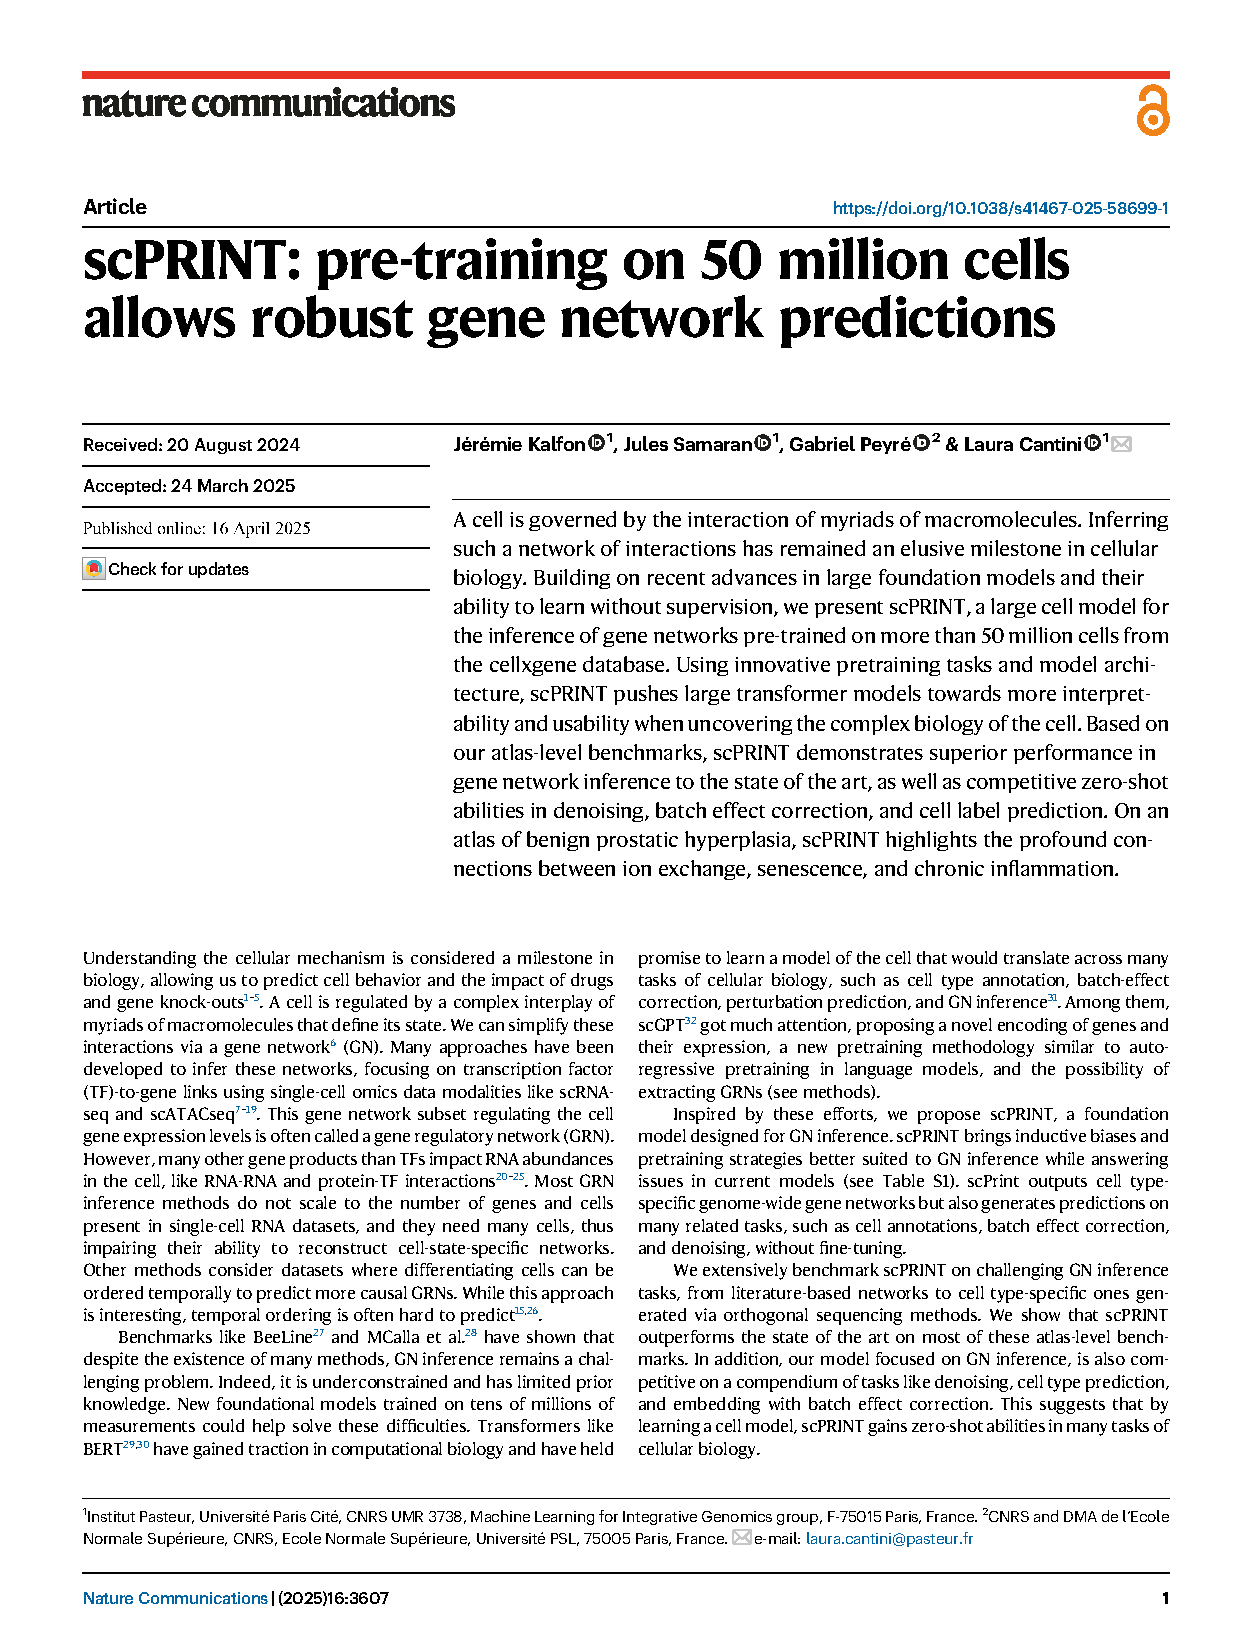
\includepdf[pages=-]{chapters/scprint.pdf}